\documentclass[smallextended]{svjour3}       % onecolumn (second format)
%\documentclass[twocolumn]{svjour3}          % twocolumn

\smartqed  % flush right qed marks, e.g. at end of proof

\usepackage{graphicx}

\begin{document}

\title{Exploring and optimising pandemic response policies with a stylised agent-based model}
%\subtitle{Do you have a subtitle?\\ If so, write it here}

%\titlerunning{Short form of title}        % if too long for running head

\author{Jeonghwa Kang          \and
        Juste Raimbault
}


\institute{J. Kang \at
              CASA, UCL \\
           \and
           J. Raimbault \at
              LASTIG, IGN-ENSG\\
              \email{juste.raimbault@ign.fr}
}

%\date{Received: date / Accepted: date}
% The correct dates will be entered by the editor


\maketitle

\begin{abstract}
% In recent years, the world has been affected by the massive spread of COVID-19 without knowing when it will end. By the time COVID-19 broke out, most countries did not have proper preparedness when the number of infected cases had started rising. This research combined an agent-based model with a compartmental model known as the SIRV to study the spread and control of epidemics. The model is used to study the effectiveness of different vaccination rates, infectious periods, immunity periods and social distancing levels in controlling epidemics during the first year of the outbreak. This research's primary analysis and learning methods include the NSGAII for parameter optimisation, Saltelli global sensitivity analysis for impact assessment of the input parameters, linear regression, and a random forest for forecasting the parameter outcomes. Also, the random sampling methods used in the analysis involve the LHS and Direct Sampling. As a result, all the model's target input parameters significantly impacted the overall infected cases. Among the input parameters, the infectious period had the most impact on the spread of infectious diseases. A longer infectious period greatly stimulated the spread of infectious diseases. In contrast, the rest of the input parameters, including the vaccination rate, immunity period and social distancing level, indicated that the higher the values, the better the suppression of epidemics.
\keywords{First keyword \and Second keyword \and More}
\end{abstract}







\section{Introduction}

The impact of one of the fatal epidemics in history, the Black Death, has led to the death of almost one-third of the population of Europe, and the most recent epidemic in the world today, COVID-19, is currently costing millions of valuable human lives \cite{glatter2021history}. Before the introduction of mathematical and computational modelling, humans had little knowledge of effectively controlling and minimising the spread of infectious diseases. Furthermore, the importance of forecasting the spread of diseases in recent years has become even more crucial as the world is rapidly globalising and becoming closer with ever-advancing technologies that make it easier for humans to travel faster and further around the globe \cite{saker2004globalization}.

The first modelling approach to disease spreading was in the 17th century as John Graunt  conducted an empirical study on infections affecting individuals in various regions in Britain \cite{morabia2013epidemiology}. Bernouilli introduced in the 18th century an equation-based approach to studying the outbreak of the smallpox epidemic in Europe\cite{dietz2002daniel}.
%In the 19th century, various mathematical equational models were further developed for modelling the complex spread of infectious diseases. The well-known equational models include the Ordinary Differential Equations (ODEs), Partial Differential Equations (PDEs) and Differential Equations. In recent years, Agent-Based Modeling (ABMs) has combined traditional equational models to study complex spatial dynamics of epidemics. After several devastating epidemic outbreaks, particularly the SARS, MERS, and COVID-19, in the recent 21st century, many models have played a vital role in developing essential government policies to counter the epidemic outbreaks from their emergence in a particular country to the current global pandemic. For example, the early spread of the COVID-19 pandemic has led to travel restrictions and closures of the countries’ borders. Monitoring the impact of various preventive measures, such as social distancing or movement policies, has been crucial in evaluating these decisions. However, strict long-term restriction policies had other devastating impacts on local and global economies. Economic evaluations and government policies have combined both economic and epidemic models to assess the economic consequences of COVID-19, informing policy calls for easing restrictions on a situational basis. At the same time, the models for social contact and mobility, have provided practical ways to evaluate appropriate pathways to reduce regulations for mobility and distancing measures safely. Finally, the advancement in agent-based modellings has provided flexibility in evaluating the dynamics of epidemics under various complex scenarios. These include examples of how governments can achieve mass immunisation or suppression of rapidly growing epidemics by introducing different vaccination strategies. Today, the methods of infectious morbidity forecasting were able to advance quickly due to the recent deployment of information supervision systems and a vast volume of statistics available for analysis. Out of all, human interaction is the most crucial factor which plays a significant role in transmitting the virus from one to the other. Interestingly, its dynamic can be modelled via a combination of ABM and compartmental model representing Spatio-temporal features in different stages of the agents during the infection process, e.g., an ABM composed of the Susceptible-Infected-Recovered (SIR) or the Susceptible-Exposed-Infected-Recovered models (SEIR) compartmental model, to name a few.
Most recent modelling approaches range from elaborated mathematical models to data-driven microsimulation models.



Beyond the health disease of epidemics, many dimensions of social systems are affected, with for example broad economic impacts \cite{boucekkine2021economics}. The current world is a highly complex systems in which various factors will play a role in decision-making \cite{bickley2021does}.
Agent-based modelling are proposed by some researchers as a powerful tool to explore practical scenarios for decision-making when managing the spread of infectious diseases \cite{miksch2019should}.

% research question
%The main objective in keeping humans safe against fatal disease outbreaks is to control the spread of infectious diseases successfully. The first step to successfully controlling the spread of diseases would be to identify which factors are likely to impact the dynamics of the epidemics. For instance, we might be interested in the effects of social distancing and wearing masks since they are well-known preventive measures that effectively mitigate the virus’s spread (Kwon et al., 2021). Furthermore, we might also be interested in the effects of vaccination since the high rate of immunisation is known to successfully control the spread of diseases and even achieve herd immunity by mass immunisation (Bicher et al., 2022). This research is generic and stylizedfor studying the spread and control of contagious respiratory illnesses such as COVID-19 and Influenza. Because the model is rather generic, it is flexible in simulating various scenarios that consider different types of infectious diseases with particular social and geographical contexts.

% This leaves us with several important research questions to answer.
%What factors affect the spread of infectious diseases, and how can we estimate the impacts of those factors?
%To what extent do different preventive measures protect humans against the spread of infectious diseases?
%To what extent do different longevity of immunity and infectious periods of the human body affect the spread of infectious diseases?
%To what extent do the optimal values of the chosen factors control the spread of infectious diseases during the first year of the outbreak?

%Questions like these are worth considering as they often come into play when recognising the importance of modelling epidemics. Guided by these research questions, there are several objectives which we list according to the analytical steps in this research:
%1. Implement an ABM that adapts the compartmental model’s dynamics to monitor and track the spread of infectious diseases in a hypothetical scenario.
%2. By using the LHS for generating random values of the model’s input parameters, explore the output space of the model by analysing the statistical distributions.
%3. Using the Grid Sampling to evaluate every possible combination of the model’s input parameter values, identify which combination results in the highest and the lowest proportional numbers of sick agents.
%4. Using the Saltelli sensitivity analysis, calculate sensitivity indices for each model input parameter.
%5. By using NSGAII multi-criteria calibration method, optimise the model input parameter values relative to the proportional number of sick agents.

%1.3 Project Scope
%This work aims to analyse and quantify the impacts of the chosen input parameters of the model on the spread of infectious diseases. The simulation projects a real-life situation where agents commute from home to their designated workplaces via different modes of transportation on a fixed daily schedule. At the beginning of the simulation, the entire population is set to susceptible. Then, an infected agent is introduced daily for the first 30 days because if none of the infected agents gets introduced into the environment, the infection process does not happen. The model’s output parameters include the number of agents associated within each state of the compartmental model upon which the ABM is based. Since the ABM is based on the SIRV compartmental model, proportional numbers of susceptible, infected, recovered, and vaccinated agents have been collected accordingly. Several analysis methods used in this research include the NGSAII for parameter optimisation (Pareto Front) and the Saltelli global sensitivity analysis for calculating sensitivity indices for the model’s input parameters. The LHS and Direct Sampling methods based on the uniform distribution are used for randomised sample selection.




%Dynamics of the ABM and Compartmental Model
%Chumachenko et al. (2018) define Agent-based modelling as ‘a relatively new direction in simulation, which is used to study the decentralised systems, the dynamics of functioning of which is determined not by global rules and laws.’ As the statement implies, the main advantage ABMs offer is an understanding of the unbiased dynamics of functioning. Its’ main aim is to understand these global rules based on the assumptions and interactions of the individuals in the system.
%The SIR model, which Kermack and McKendrick initially introduced in 1920, is often applied to the mathematical modelling of infectious diseases. This model for influenza describes the process of disease transmission in various states. For example, (S) stands for susceptible, (I) for infected, and (R) for recovered states of the agents in the model. Chowell, Miller and Viboud (2008) use the SEIRD compartmental model to study the spread of influenza in three countries: the U.S., France, and Australia. The SEIRD model is an advanced version of the traditional SIR model, consisting of individual agents exposed to the diseases but not exhibiting symptoms yet. Also, this model considers the death of agents in the population. To better understand the model's dynamics, the SEIRD model is demonstrated below,
%[ eqs seird]
%For example,,, and indicate the numbers of exposed, immune, and dead individual agents respectively. The shows the transmission rate, and �� is the total population. denotes the rate at which respective agents go from exposure to infection. Lastly, �� and �� indicate the recovery and mortality rates, respectively. Using this SEIRD compartmental model, Chowell, Miller and Viboud (2008) study the effectiveness of vaccination in spreading and controlling influenza. They concluded that a higher vaccination rate of susceptible agents is necessary to prevent and effectively reduce the spread of flu. Furthermore, they found that the re-vaccination process would further enable better control of the diseases. Another approach to modelling the spread of infectious diseases comes from a discrete model (Difference Equation). This model determines the variable quantities at distinct time intervals. Hence, this approach is well suited to representing the time series data. For example, the SIR compartmental model in the discrete form is shown below,
%[]
%In the equation, ���� , ���� , and ���� indicate the number of susceptible, infected, and recovered individual agents at time �� respectively. �� indicates the number of contacts and �� represents the birth and death rates. Lastly, the �� refers to the recovery rate. Ramani et al. (2004) used discrete-time models to study the spread of epidemics over time under two different scenarios. The first scenario assumes no changes in the number of total populations with no occurrence of death. The second scenario assumes that the total number of population changes either by permanent recovery or death of agents. For the first scenario, the number of infectiousdiseases reached a fixed point without disappearing. However, according to the second scenario, where individual agents are allowed to leave the population by means of death or permanent immunity, the epidemic often died out completely in the simulation.

%The models mentioned above are all examples of traditional models. Therefore, they often pose limitations compared to the most recent Agent-Based Model. The main limitation is that traditional models fail to describe agent behaviour variations accurately. To overcome the limitation, Chumachenko et al. (2018) proceeded to advance the model by combining the concept of the SIR compartmental model with an ABM to study the spatial aspect matter in propagating epidemics. This type of modelling is a relatively new study area compared to traditional modellings. The ABM’s environment comprises grid cells or patches where individual agents reside. These patches are where the agents contact each other and interact with the environment. The models’ patches and agents may have specific features. For instance, patches may have attributes that can affect agents’ movement or interactions. We can also define characteristics such as location, age, and many other factors believed necessary in the model for each agent. Once the agents are defined with their own set of characteristics, they proceed through a set of rules which enable them to interact with other groups of agents within the simulation. The agents’ range of interactions may differ depending on the model types. For instance, in predator-prey models, one kind of agent may feed off another, while in competition models, agents with entirely different properties may compete for survival. In epidemic models, infected agents may infect other susceptible agents through interaction. Furthermore, adapting the compartmental model into the ABM advances the epidemic model by adding multiple states of agents, generating much more detailed simulation results.

% The Interactions and Infections
%The characteristics of agents are important in studying and forecasting the spread of diseases as they determine how contacts and infections between the agents occur in a simulation. Chumachenko et al. (2018) define two agents: the ‘age-human’ and ‘location-human’. Firstly, the age of an agent determines the probability of contact between agents. Changes in the value of the contact rate would also affect the infection rate. There are five age groups: children, teens, youth, adults, and elderly. Among the group, both children and elderly groups are deemed to be in contact with fewer people than younger groups. Also, the communication between the agents is made if they are located on the same patch only. This is mainly to reduce the computational complexity of the model by controlling the agents’ interactions per patch instead of considering multiple neighbouring patches altogether. Reducing the computational cost for simulation is a crucial factor, especially for the ABMs, since the cost may increase when there are many combinations of the variables to consider per execution. Because the research depends on developing the ABM on Netlogo, minimising the computational complexity is crucial for the system’s smooth operation since the Netlogo modelling environment is mainly for educational purposes rather than advanced research.

%Minoza, Bongolan and Rayo (2021) introduce several essential variables that describe the agents’ characteristics, including age, status, wearing face masks, physical distancing, lockdown and immunity. Depending on the age of an agent, the probability of contact differs among the agents. The variable that checks whether a susceptible agent is wearing a mask during the interaction with an infected agent may well reflect a real-life situation. Hence, this can be a good consideration factor for calculating an accurate infection rate that can better shape the disease transmission dynamics. The immunity variable here indicates if an agent is permanently immune or not. The limitation with the SIR or SEIR model is that once an agent fully recovers from infection, the agent is considered permanently immune throughout the simulation. However, this does not correctly depict a real-life situation as immunity against most infectious diseases is impermanent. Therefore, the immunity period of an agent should be re-constructed in a way that is not permanent; hence, if a specific time passes, the agent becomes susceptible and vulnerable to infection again. To go a step further, a variable that defines an agent’s medical conditions can play an essential role in determining a reliable infection rate as it is known that a person who is suffering from cardiovascular diseases is at a high risk of getting infected, mainly due to a defeated immune system (Fekadu et al., 2021). The properties of agents that can impact the infection rate should carefully be considered based on the interest of the research topic, as they play an essential role in shaping the overall outcome of a simulation.

% Vaccination and Immunity
%Kaszowska-Mojsa, Włodarczyk and Szymańska (2022) carried out an analysis of the impact of the COVID-19 outbreaks on labour productivity by comparing the results obtained from three different scenarios using the dynamic stochastic general equilibrium model with an agent-based epidemic component. The paper indicates the effectiveness of vaccines in association with various preventive measures such as lockdown, quarantine, and social distancing against the spread of the virus in a hypothetical simulation. Furthermore, the scenarios in this paper introduce different levels of restrictions to control the spread of COVID-19. For instance, scenarios with varying intensity levels of lockdown, quarantine, and social distancing with and without vaccination in a simulation were tested, and the results were compared. The conclusive results indicate that the vaccination process is crucial in controlling epidemics’ spread. It is concluded by the findings that the effectiveness of the lockdown, quarantine, and social distancing alone could not achieve herd immunity even though such procedures may temporarily slow down the general spread of diseases. For a community to achieve herd immunity, it has been found that approximately 90\% of the population must be vaccinated or naturally immunised from recovery. This process can be fastened if the effectiveness of vaccines and the probability of agents receiving the vaccines increase. Physical well-being is also a crucial factor that ensures society’s safety from harmful diseases, but the importance of healthy economic growth cannot be neglected either. Therefore, policymaking during a pandemic would be challenging in a situation where human lives and the economy are at stake. As a result, the restrictions such as lockdown and quarantine will eventually get lifted, and the preventive measures will be eased once humans know how the spread of diseases can be controlled and prevented. In conclusion, the right approach would be to keep focusing on evaluating the impacts of various preventive measures against such diseases and finding the optimal solution sets that can effectively control disease spread.

% Assessing the Impacts of Model’s Input Parameters
% Baquela and Olivera (2022) utilises one of the multi-objective evolutionary algorithms (MOEA) for optimising the distribution of limited COVID-19 vaccines across the provinces in Argentina. The distribution of vaccines is prioritised among different groups of the population. The group with the highest priority comprises the older people and medical workers, who comprise about one-third of Argentina’s total population. Then, the overall distribution of the vaccines across geographical groups is indicated by the average Gini coefficient. A value close to zero Gini coefficient indicates perfect equality. In this case, having a zero Gini value would mean all the vaccines are equally distributed throughout the provinces in Argentina. A value close to one would mean the distribution of vaccines across the provinces in Argentina is entirely biased. Baquela and Olivera (2022) denote that the usual way to group the population is based on the severity of infected cases, the standard criterion most governments depend on to define priorities for vaccination during the COVID-19 pandemic. However, this is not always the case for countries like Argentina as there are multiple issues to consider, such as logistic issues to distributing vaccines and legal and ethical issues. Due to these, one cannot simply supply a high number of vaccines to some provinces while keeping other regions without vaccines. Furthermore, vaccines are expensive, and certain countries cannot bear the costs of these vaccines to cover their entire population. This is known to further damage the economy since the ways to control the spread of infectious diseases in countries without vaccines are heavily dependent on isolation policies (Hafner et al., 2020). This is where multi-objective evolutionary algorithms can help solve problems that pose many conflicting objective functions. NSGAII applies Pareto dominance for the fitness calculation, building fronts of solutions. The Pareto Front refers to a set of optimal solutions which are non-dominant to each other but are superior to the rest of the solutions in the search space (Yusoff, Ngadiman and Zain, 2011). However, the Pareto front does not identify how much variations in the model’s input parameter affect the variations in the model output parameters. One way to tackle this problem is by conducting sensitivity analysis which acts as an in-depth study of all the model variables. Conducting sensitivity analysis is useful, particularly for decision-makers. The results obtained by such analysis are far more reliable in the sense that it quantifies the impacts of the model’s input parameters by calculating the changes in the total variance of the model’s output parameters, thereby identifying where they can make improvements to obtain better results in the future (Saltelli, 2008).

%Wu et al. (2013) developed a model of infectious diseases based on a compartmental model which consist of six compartments: susceptible, exposed, infected, recovered, dead and vaccinated. The model has been parameterised to model a disease outbreak in a large metropolitan area. These input parameters include age, contact rate, quarantine effectiveness rate, disease infectivity rate, vaccine effectiveness rate, and fatality rate. In order to quantify the impacts of each input parameters, Saltelli’s global sensitivity analysis is applied to the infection model. This type of analysis is used to determine how much of the variability in model output is dependent on each of the input parameters, either upon a single parameter or interaction between different parameters (Zhang et al., 2015). For instance, if one of the input parameters has a small value of the sensitivity index, it indicates that the variation of this parameter is most likely to result in a slight variation in the output parameters. On the other hand, if the sensitivity index is high, a change in the value of the input parameter will likely lead to a dramatic change in the output parameter values. The sensitivity analysis can, therefore, guide experimental focus so that researchers can take special care in obtaining more precise and reliable measures of parameters by referring to these sensitivity indices.

%As discussed above, it has proved to be quite effective in modelling the spread of infectious diseases in various compartmental models such as the SIR and the SIRV. These models, in general, allow for a detailed evaluation of various preventive measures such as vaccination rates, quarantine, social distancing or lockdowns as one of the model's input parameters on the spread of epidemics. Various compartments precisely describe each state of an agent in the infection process and provide solutions to control the spread of epidemics effectively. Furthermore, the advantage of using these models is that they provide a better representation of the data because data gets collected in discrete time intervals. On the other hand, they pose limitations too. One of the limitations is that they are not suitable for collecting Spatio- temporal data. Hence, these models ignore the spatial aspects of the infection dynamics. The spatial data is as significant as the temporal data in the field of epidemiology because the infection dynamics can vary greatly depending on different spatial structures of the environment. As a solution, the ABM can combine one of the compartmental models mentioned earlier to overcome these limitations. Since the effectiveness of vaccination is one of the main interests of the research, instead of adopting the traditional SIR model, we can base the SIRV model on our ABM to consider the vaccination state of the agents in the simulation. This way, the model collects not just the temporal data but also the spatial data as an outcome of the simulation. Various methods have been mentioned earlier regarding the analysis tools, including the NSGAII for parameter optimisation and Saltelli for global sensitivity analysis, to name a few. One thing to note is that this research should not stick to just one analysis method to assess the overall impacts of the model's input parameters. Instead, we combine the analysis methods. The NSGAII to obtain the optimal set of the input parameter values that best control the spread of epidemics and Saltelli global sensitivity analysis to find out which model input parameter significantly affects the overall output parameters. Also, training a random forest learning algorithm is an excellent way to forecast the outcome of our ABM simulation and assess how well the model can predict the spread of infectious diseases. Through the random forest model, we can also calculate the importance of each input parameter and compare the result with the result obtained by Saltelli sensitivity analysis. In order to visualise the statistical distribution of the model outputs, random sampling methods such as the LHS and direct sampling, which select samples based on uniform distribution, can be adapted in the analysis process. Lastly, linear regression is also proven to be an effective tool for predicting the dependent variable, which is the proportional number of sick agents in our case. Coefficient values of the input parameters can be calculated using this tool and estimate the impacts of each of these parameters on the dependent variable.


\section{Model description}


\subsection{Model setup}

%The main interest of this research is investigating the effectiveness of various pre-defined model input parameters on spreading and controlling infectious diseases that result while the agents are commuting from home to the workplace. This model assumes that most human interactions occur while people travel and work. Hence, the scenario is primarily about people commuting from home to their designated workplaces via different modes of transportation, closely depicting ordinary people's daily routine. Using NetLogo, the model is tested on a 2D environment where agents representing people are distributed homogeneously throughout. The simulation of this model considers several essential assumptions. The entire duration of the simulation is set to 365 days. Each day is equivalent to 24 ticks. Hence, each tick is equivalent to an hour. A single day comprises three pre-defined phases: the ‘Home-hour’, ‘Commute-hour’ and ‘Work-hour’ phases. Each phase is indicated by different colours of the patches in the simulation; orange indicates the ‘Home-hour’ phase, black for the ‘Commute-hour’ phase and cyan for the ‘Work-hour’ phase.
\begin{figure}
	\centering
	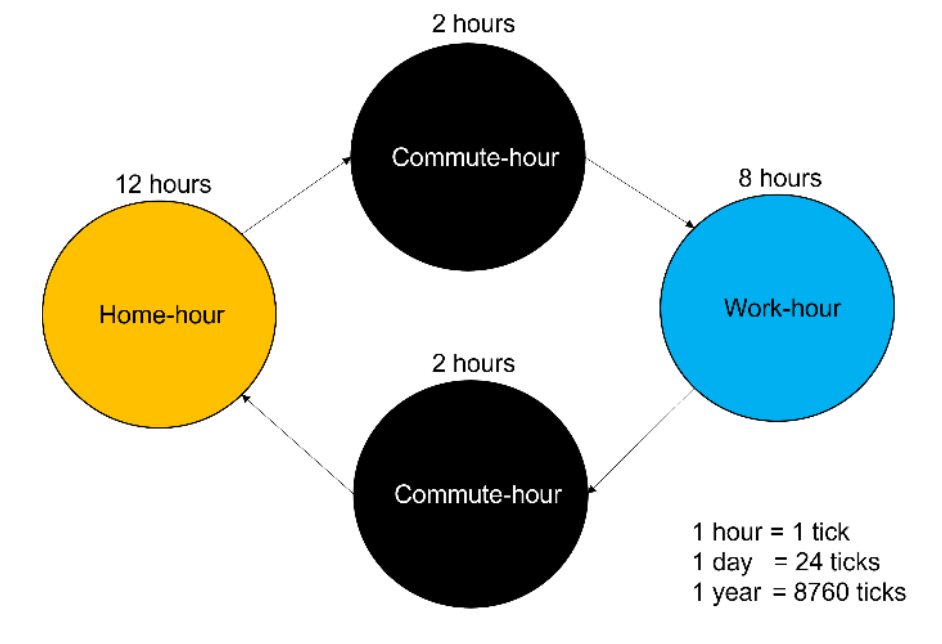
\includegraphics[width=0.5\linewidth]{figures/ModelTransitions.png}
	\caption{TRANSITION OF THE PHASES IN THE MODEL}
\end{figure}

%During these phases, the movement of agents is completely randomised. No learning behaviour alternates the agents’ movement in the simulation since it would be difficult for an individual to be fully aware of another agent’s infection status. During the interaction, agents fall into one of the four states defined by the SIRV compartmental model, which this research’s ABM is based upon. The SIRV model is an extended SIR model that accounts for the vaccination of the susceptible population \cite{poonia2022enhanced}.
\begin{figure}
	\centering
	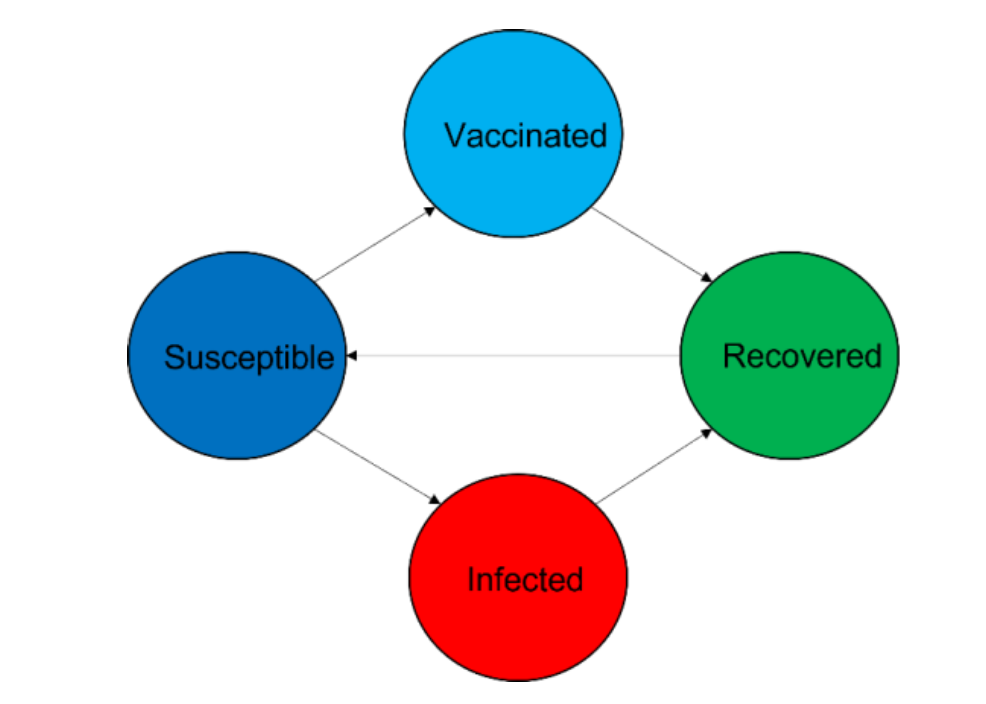
\includegraphics[width=0.5\linewidth]{figures/AgentStates.png}	
	\caption{Agent states in the model\label{fig:agentstates}}
\end{figure}

%Agents can interact with each other based on the state in which they fall. However, the interaction and infection processes are set to occur between the agents within the same patch only. The infection does not happen during the 'Home-hour' phase as this model does not consider social activities or household infections. During the 'Commute-hour' phase, an infected agent can only infect the susceptible agents that use the same mode of transportation as itself. It would be logically sensible that an infected agent commuting via train can only interact with and infect other susceptible agents commuting via the same mode of transportation. This same logic applies during the 'Work-hour' phase, where an infected agent can only interact with and infect other susceptible agents working in the same company. The following table lists all the modes of transportation and the names of companies defined in our model.
Modes
of Transportation Bus
Tube
Train
Walk
Car
Big-sized
Companies
Apple
Google
Amazon
Facebook
Samsung
Toyota
Coca-Cola
Mid-sized Companies
Small-sized
Companies
    Yahoo NHS
    Dell
Zara GAP
Sainsbury Tesla H\&M
[Table 1]

%The actual company names are used here to assign each agent’s company variable. There are total of fifteen companies which are randomly categorised into small, mid, and big-sized companies. The central assumption is that the bigger the company size, the more the human interactions involved. Hence, the agents working in a big-sized companies are more likely to get infected than the agents working in mid and small-sized companies.

At the beginning of the simulation, 1500 susceptible agents are randomly distributed in the simulation environment. The variable values for the agents, such as the transportation and company, are randomly assigned during the setup stage. An infected agent is then constantly introduced at a random location for the simulation's first month (30 days). Every day, a random percentage value from zero to one percent of the total population gets replaced. This is based on the assumption that the population is dynamic. A certain number of people leave the area, and others come to stay in the area. Hence, the total population is not fixed to the initial population throughout the simulation.


\subsection{Model parametrisation}


\begin{figure}
	\centering
	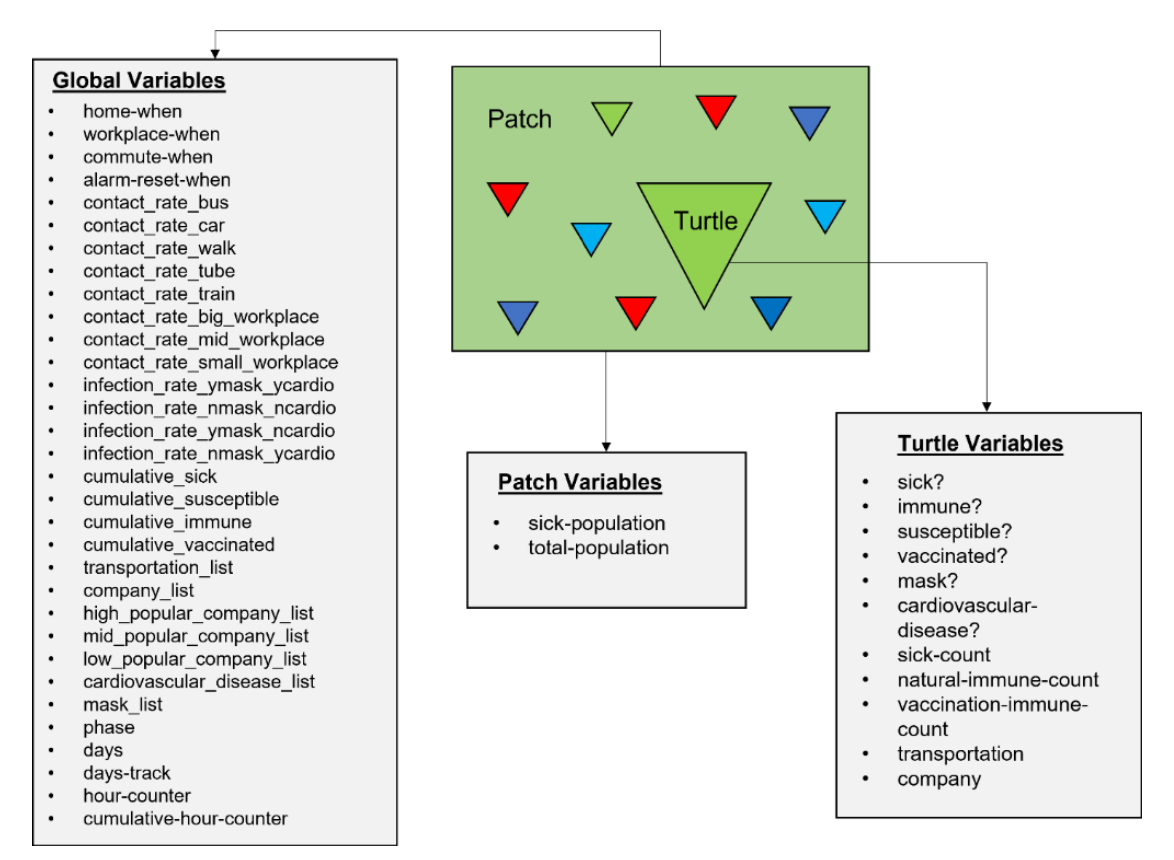
\includegraphics[width=\linewidth]{figures/ModelVariables.png}
	\caption{Model variables \label{fig:modelvars}}	
\end{figure}



\subsubsection{Global variables}

Infection rates are calculated based on the values of the global, patch and turtle variables. The variables that define contact rates for each mode of transportation and company are pre-defined with specific values.

For transportation contact rates, we take stylised values decreasing with the density one can expect in each transport mode: $c_{bus} = 40\%$, $c_{metro} = 35\%$, $c_{train} = 30\%$, $c_{walk} = 10\%$, $c_{car} = 10\%$.

No discrete values define the accurate contact rates for different modes of transportation, but the general assumption was made based on the understanding that the lower the capacity of transportation, the higher the density; hence, the higher contact rates between the passengers. The contact rate specifically for the car is set to zero because it is assumed that an agent who commutes by a car makes no contact with other agents during the 'Commute- hour' phase. The same logic was applied when defining the contact rates for different companies. The assumption was based on the understanding that the bigger the company size, the more the agents interact.

For contact rates on work site, we therefore take the following values: $c_{Big} = 40\%$, $c_{Medium} = 35\%$, $c_{Small} = 30\%$


\subsubsection{Agent variables}


• mask?
• cardiovascular-disease?
As discussed in the literature review, the importance of wearing a mask while interacting with an infected agent can significantly reduce the chance of infection. Furthermore, patients with cardiovascular diseases are known to be at high risk of getting an infection. Due to these reasons, we have pre-defined values for infection risk rates based on the combination of these two variables.

Conditions
No mask \& Cardio
No mask \& No Cardio
Mask \& Cardio
Mask \& No Cardio
Infection Risk Rate
50 %
45 %
15 %
10 %
TABLE 4. RISK RATES FOR COMBINATIONS OF THE MASK AND CARDIO VARIABLES



[Patch variables]

• sick population
• total population
For each patch, the values of the sick and the total population get updated constantly. If the value of the sick population gets bigger than zero, the infection process between the agents within that specific patch gets triggered.


\subsection{Model parameters}

\begin{itemize}
	\item Infectious period, ranging from 2 to 4 weeks; the longevity of the infectious period of an agent is believed to play an essential role in the spread of diseases because the longer the infected agent stays contagious, the more the chance of infection during an extended amount of time \cite{wilkinson2018impact}.
	\item Immunity period, ranging from 9 to 11 months. This is selected as one of the model’s input parameters because it is believed to play a vital role in protecting the agents from infection \cite{reyes2016modeling}. Hence, we are interested to know to what extent the immunity period significantly affects the spread of diseases.
	\item Vaccination rate: as discussed in the literature review, vaccines are the most effective preventive measure which can trigger a biological immune response to fight disease-causing organisms. The value ranges from 0 to 0.5 \%, meaning from 0 to 0.5 \% of the susceptible population is set to be vaccinated daily. A high vaccination rate is strongly believed to be the key to the successful control of epidemics; hence, finding out the impacts of different vaccination rates on the overall infection process would be meaningful.
	\item Social distancing level: a certain level of social distancing is being applied by governments worldwide, hoping to stop the spread of diseases like COVID-19. However, the effect of social distancing is not yet well known. Due to this, it would be an interesting experiment to find out the effectiveness of such measures on disease transmission dynamics. The level of social distancing ranges from 1 to 3. Each level refers to a percentage value that reduces the contact rate by 5. Hence, the actual percentage value of the social distancing ranges from 5 to 15 percent. The higher the intensity of social distancing, the lesser the chance people contact each other.
\end{itemize}



\subsection{Model indicators}


• A proportional number of sick agents
• A proportional number of immune agents
• A proportional number of susceptible agents
• A proportional number of vaccinated agents
As mentioned previously, the ABM is constructed under the concept of the SIRV compartmental model. Therefore, the results consist of proportional numbers of agents in each compartment, including susceptible, infected, recovered, and vaccinated.
For demonstration purposes, we calculate,
• The infection rate for agents who commute by train during the 'Commute-hour' phase
• The infection rate for agents who work in the 'Apple' company during the 'Work-hour'
phase.

%The calculations for the rest of the infection rates follow the same process illustrated by the demonstration. Hence, this research demonstrates one exemplary calculation for each phase. To calculate the infection rate among the agents who commute by train in each patch, Let, the number of sick agents whose mode of transportation is train, 𝑆𝑡 Let, the total number of agents whose mode of transportation is train, 𝑃 𝑡 Let, the contact rate of the train, 𝐶𝑡 Let, the level of the social distancing, 𝐷 Let, the infection risk rate, 𝑅 Toobtaintheproportionalvalueof𝑆 to𝑃, 𝑡𝑡 𝑀𝑡 = 𝑆𝑡 𝑃𝑡 To obtain the infection rate of train 𝐼𝑡, 𝐼𝑡 = 𝑅(𝑀𝑡𝐶𝑡 − 0.05𝐷)
%To calculate the infection rate among the agents who work in Apple in each patch, Let, the number of sick agents who work in Apple, 𝑆𝑎 Let, the total number of agents who work in Apple, 𝑃 𝑎 Let, the contact rate of big-sized company, 𝐶𝑏 Let, the level of the social distancing, 𝐷 Let, the infection risk rate, 𝑅 To obtain the proportional value of 𝑆 to 𝑃 , 𝑎𝑎 𝑀𝑎 = 𝑆𝑎 𝑃𝑎 To obtain the infection rate of Apple 𝐼𝑎, 𝐼𝑎 = 𝑅(𝑀𝑎𝐶𝑏 − 0.05𝐷) A counter variable keeps a time (tick) record as soon as an agent becomes infected. The value of the counter variable is then compared with the model’s input parameter called the 'infectious- period'. Once the counter exceeds the value of this parameter, the infected agent becomes immune. The counter variable gets reset to zero whenever an agent switches its state. The counter variable keeps a record of time (tick) again as soon as the agent becomes immune, and if the counter exceeds the value of the 'immunity-period', which is also one of the model’s input parameters, the agent becomes susceptible. The same dynamic applies when a susceptible agent becomes vaccinated. The overall dynamic of the model is further described in the diagram below and the entirety of the codes can be seen in Appendix D.


\begin{figure}
	\centering
	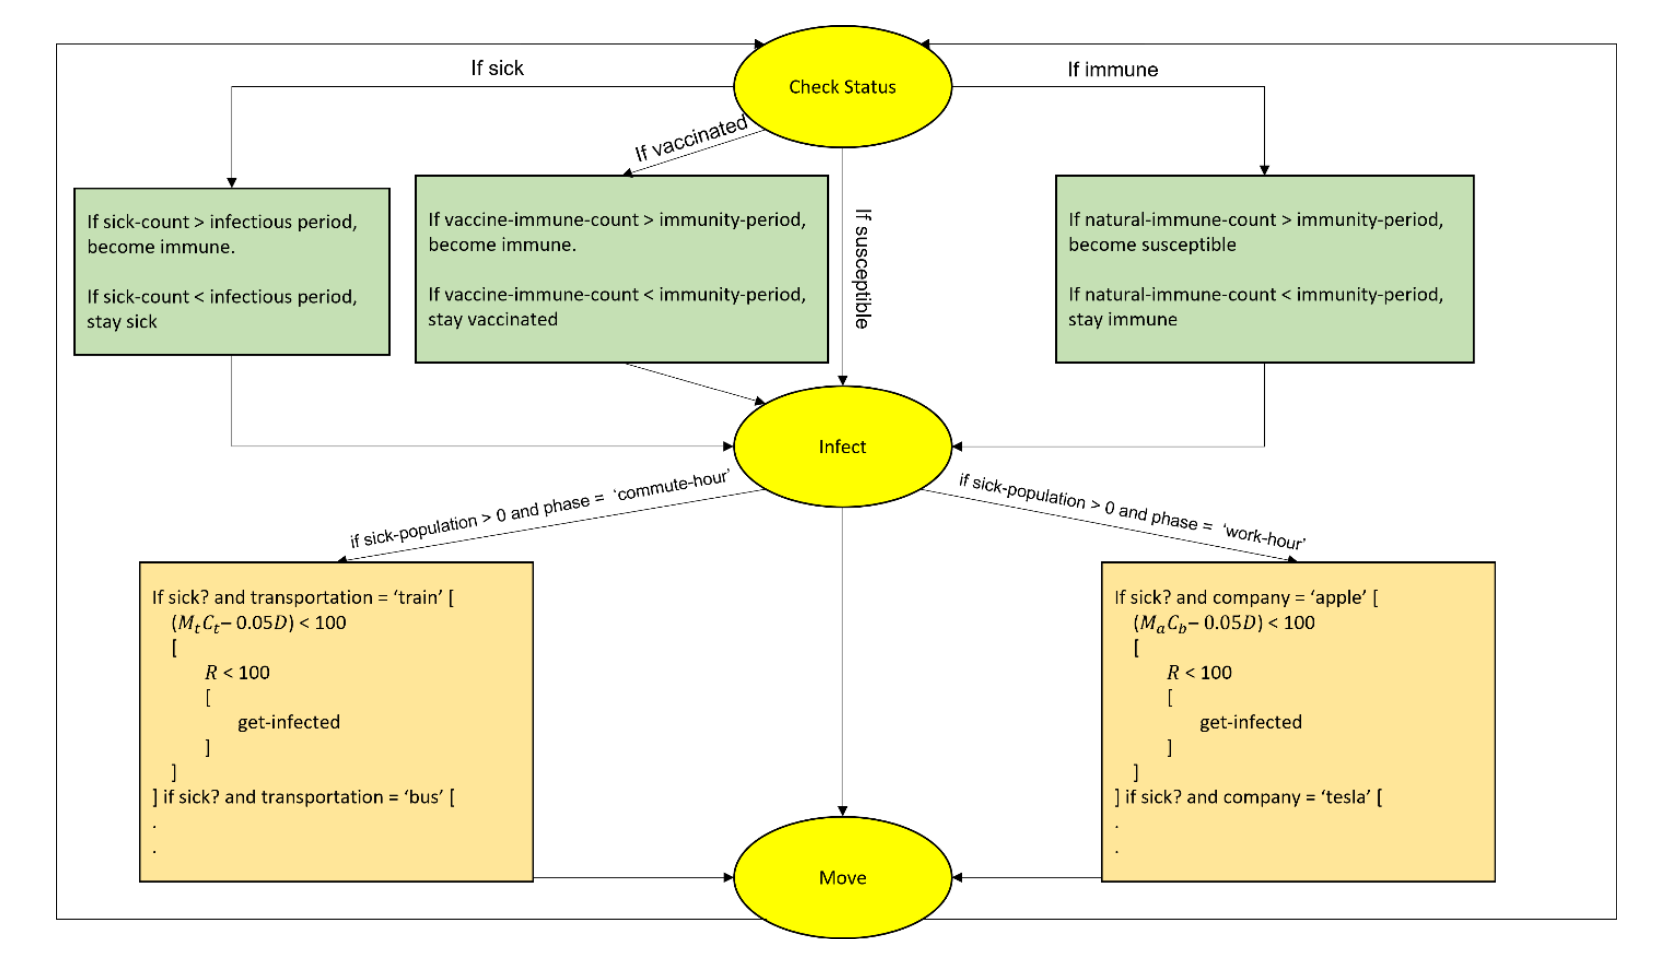
\includegraphics[width=\linewidth]{figures/modelDynamics.png}
	\caption{DESCRIPTION OF THE MODEL DYNAMICS\label{fig:modeldyn}}
\end{figure}


\subsection{Model implementation and exploration}

%3.2 Description of the Analysis
%The analysis of the model is carried out on the platform called OpenMOLE. It provides various analytical tools to run and optimise the ABM in high performing computing environments. The analytical methods, such as the Saltelli global sensitivity analysis and NSGAII, which are used as parts of the analysis, are available on OpenMOLE. The main benefit is that it allows the users to explore the models across multiple programming languages, including Java, Netlogo, R and Python. The OpenMOLE also comes with a graphical user interface to write scripts around our model, and these scripts will effectively explore the model by distributing its executions on high- performing computing environments (OpenMOLE, 2008). The scripts used in the analysis are in oms file format which can be found in Appendix D.
%3.3 Statistical Distributions of the Model’s Output Parameters
%Statistical distributions of the output parameters provide a general picture of the output space of the model. Running as many models as possible with different values of the input parameters better shapes the model’s output space and validates the results. Thus, the LHS method is used to sample ten thousand random values of the input parameters with an equal probability (McKay, 1992). To better interpret the results, graphs such as histograms for illustrating the overall statistical distributions, box & whisker for representing different data ranges and QQ plots for analysing the shapes of the statistical distributions are used.
%3.4 Grid Sampling of the Model’s Input Parameters
%A grid sampling, also known as complete sampling, is a method which is used to evaluate every possible combination of the input parameter values for a reasonable number of dimensions and discretisation step (Elementary Samplings, 2022). The primary purpose of conducting a grid sampling in this research is to find out which values of the input parameters generate the highest and the lowest proportional numbers of sick agents.
%Here are the pre-defined input parameter values of the model:
Input Parameters
infectious-period
immunity-period
vaccination-rate
social-distancing-levels
Value Range
2, 3, 4 (weeks)
4, 5, 6 (months)
0, 0.25, 0.5 (\%)
1, 2, 3 (levels)
        TABLE 5. PRE-DEFINED VALUES FOR EACH MODEL INPUTS
        
        
        This results in 81 different combinations of the input parameter values for a grid sampling. The model is set to run over 125 times for every combination of the input parameter values, and the output parameters’ average values are obtained at the end.
With the result, the average proportional numbers of sick agents are aggregated based on each value of the input parameters, as shown in Table 5 above, to explore the input space of the model. The statistical distributions of the results are presented in a box \& whisker plot.






\section{Results}


%This chapter presents the results obtained using the analytical methods described in the previous chapter. Firstly, statistical distributions of the model’s output parameters are presented with histograms and box & whisker plots. A QQ plot is also used to describe the shapes of the output distributions relative to the normal distribution. Secondly, the combinations of the input parameter value that produce the highest and the lowest proportional numbers of sick agents are identified by re-ordering the table rows. Then, the proportional numbers of sick agents that are grouped by each value of the input parameters are presented on a box & whisker plot. Thirdly, we use the correlation matrix to illustrate the relationship between the model’s input and output parameters. Linear regression analysis is supplemented to summarise the relationship between the model parameters. Fourthly, a random forest is trained with the data obtained from the LHS (refer to the first step of the analysis), and the predicted data is compared with the actual data. Lastly, the results obtained by the Saltelli global sensitivity analysis are presented in a table, and the Pareto Front, which NSGAII obtains, is presented on scatter plots.
We describe now numerical results obtained through the extensive exploration with the OpenMOLE platform.


\subsection{Statistical distribution of indicators}

The LHS (Latin hypercube Sampling) method was used to explore the input space of the model. A total of 10,000 samples were run during the process.

According to the execution time, the execution time is 4 days and 4 hours. 4 days 4 hours
%= 4.16 days 4.16 days * 24 hours = 99.84 hours 99.84 hours * 60 minutes = 5,990.4 minutes

\begin{figure}
	\centering
	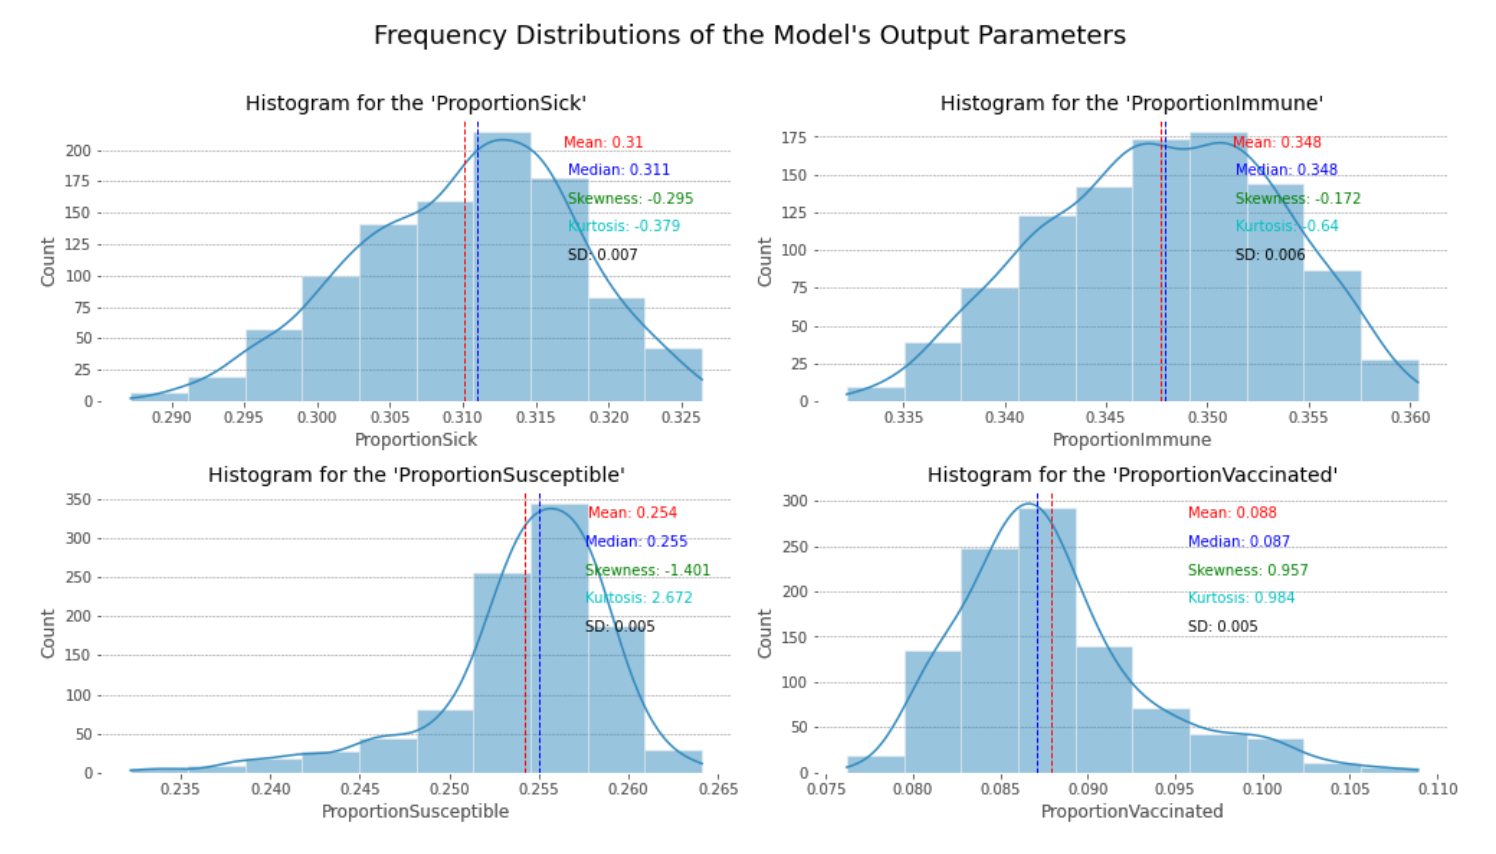
\includegraphics[width=0.7\linewidth]{figures/histograms.png}
	\caption{HISTOGRAMS OF THE MODEL OUTPUTS\label{fig:histograms}}
\end{figure}

The histograms in Figure 9 illustrate the four different output parameters of the model. The histograms in the upper row comprise the ‘ProportionSick’ and the ‘ProportionImmune’ histograms, which appear symmetrical, but the skewness values indicate the traits of negative skewness on each histogram plot. Both kurtosis values are negative, suggesting that the distributions are thin-tailed. From this finding, we can assume that they generally follow characteristics of the platykurtic distribution. The ‘ProportionSusceptible’ and the ‘ProportionVaccinated’ histograms in the lower row appear negatively and positively skewed, respectively. The ‘ProportionSusceptible’ histogram is highly skewed to the left, which is indicated by the skewness value lesser than -1, while the ‘ProportionVaccinated’ histogram appears moderately skewed to the right as its skewness value indicates slightly lesser than +1. Furthermore, the kurtosis values of the two histograms are positive, which indicates that they both have heavier tails and are likely to follow the shape of the leptokurtic distribution.


% Figure 10 : qq plots
% The QQ plots shown in Figure 10 compare statistical distributions of the output parameters of the model relative to normal distribution. The shape of the ‘ProportionSick’ distribution closely follows the normal distribution but gets steeper towards the right. The ‘ProportionImmune’ distribution resembles the 'S-shaped trajectory of the data points. This implies that the distribution has thinner tails on both sides, shaping the distribution narrower compared to the normal distribution. The ‘ProportionSusceptible’ and ‘ProportionVaccianted’ data points resemble concave downward and upward shapes relative to the normal distribution line, respectively. This implies that the former distribution is negatively skewed, and the latter is positively skewed.


\begin{figure}
	\centering
	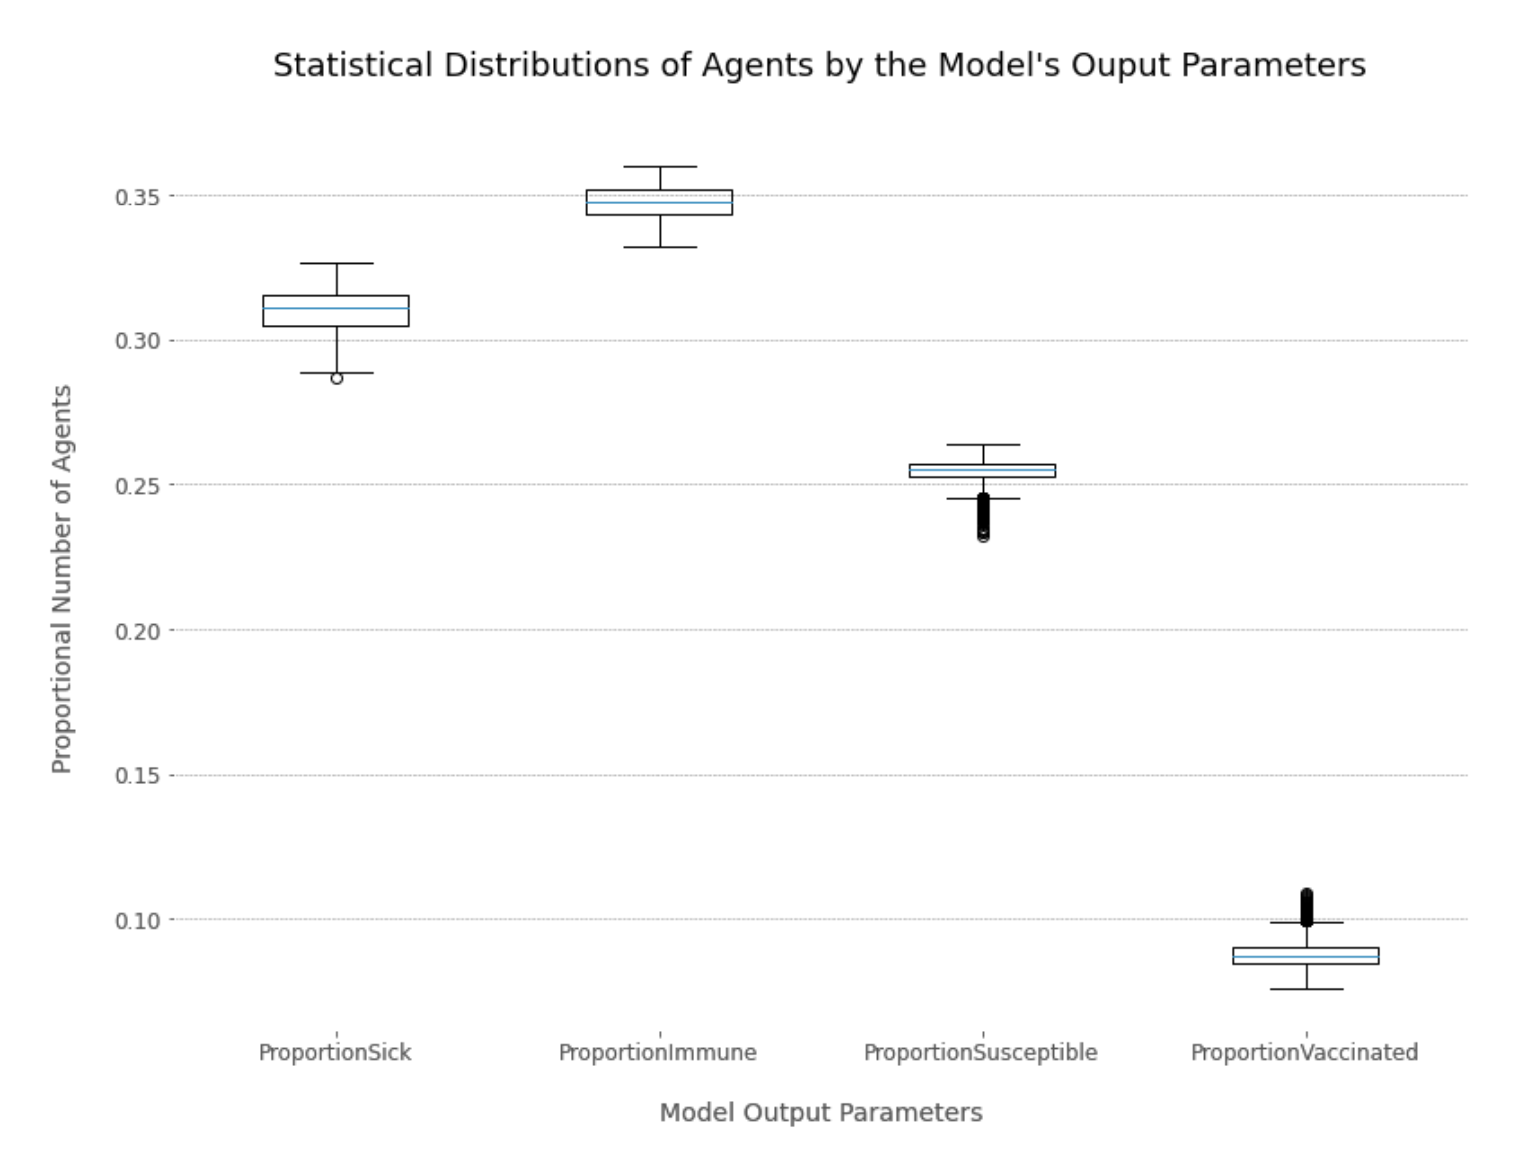
\includegraphics[width=0.7\linewidth]{figures/agentTypeDistrib.png}
	\caption{BOX PLOTS OF THE MODEL OUTPUTS\label{fig:agenttypedistrib}}
\end{figure}


The boxplots presented in Figure 11 show different data ranges and medians of the four different output parameters of the model. The boxplot representing the ‘ProportionImmune’ appears to have the highest median among the groups, followed by the ‘ProportionSick’, ‘ProportionSusceptible’ and ‘ProportionVaccinated’, respectively. Outliers in the boxplots are present regarding the ‘ProportionSusceptible’ and ‘ProportionVaccinated’. Based on the histograms shown in Figure 9, these distributions have positive kurtosis values and are disproportionally distributed, indicating low standard deviation; hence, high chance of producing outliers.


%4.2 Exploration of the Model’s Input Parameters via Direct Sampling
\subsection{Grid exploration}

The total combination of the model's input parameters is 81, as mentioned in the methodology section. The model run for each combination of the inputs is set to 125 times. This results in a total model run of 10,125, for a total execution time of 4 days and 5 hours.
%4 days 5 hours = 4.21 days 4.21 days * 24 hours = 101.04 hours 101.04 hours * 60 minutes = 6,062.4 minutes

Table 6 presents the combinations of the input parameter values relative to the five lowest values of the ‘ProportionSick’. The lowest value of the ‘ProportionSick’ among the 10,000 samples is 0.2779. The combination of the input parameter values that generated the lowest ‘ProportionSick’ is shown in the first row of the table. The ‘infectiousPeriod’ and the ‘vaccinationRate’ values remained constant at 2 (weeks) and 0.005 (0.5\%) respectively, while the ‘immunityPeriod’ and the ‘socialDistancingLevels’ varied throughout the table.

Table 7 presents the combinations of the input parameter values relative to the five highest values of the ‘ProportionSick’. According to this table, the highest value of the ‘ProportionSick’ among the 10,000 samples is 0.3280. The ‘infectiousPeriod’ and the ‘vaccinationRate’ remained constant at 4 (weeks) and 0.0 (\%), respectively, while the rest of the input parameter values varied throughout the table.




\begin{figure}
	\centering
	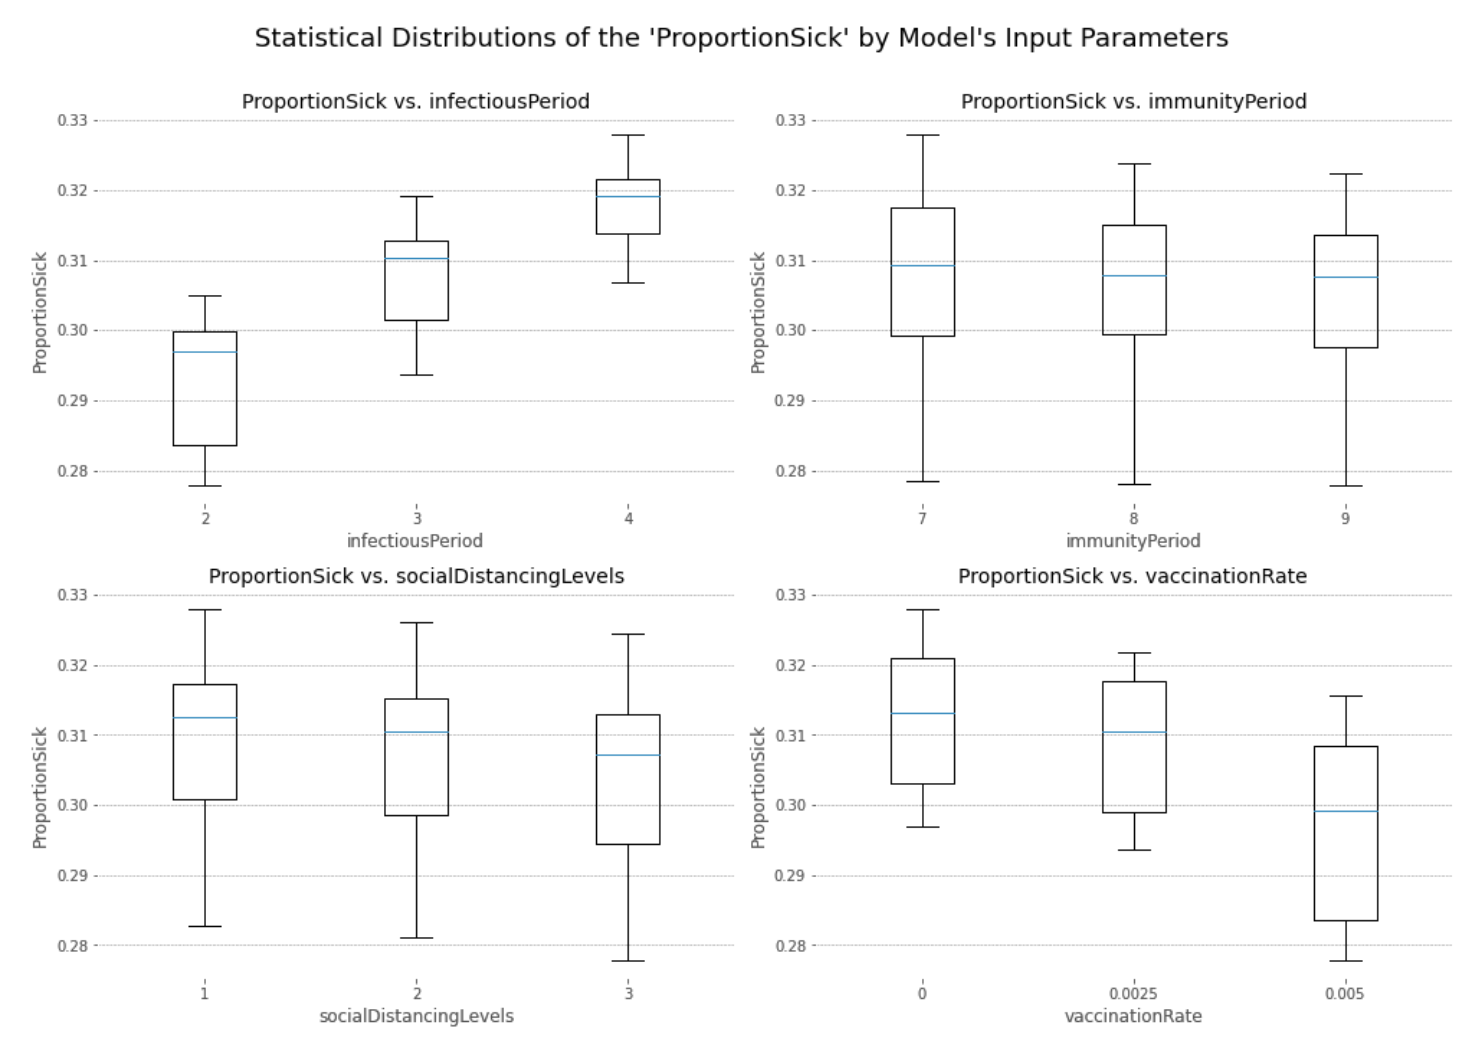
\includegraphics[width=0.7\linewidth]{figures/boxplots.png}
	\caption{BOX PLOTS SHOWING AGGREGATE VALUES OF THE MODEL OUTPUTS BASED ON EACH VALUE OF THE MODEL INPUTS\label{fig:boxplots}}
\end{figure}


The box plots in figure 14 show statistical distributions of the ‘ProportionSick’, which are grouped by each input parameter value of the model. The range of each input parameter is indicated on the horizontal axis of the graphs.
The first graph represents the grouped values of the ‘ProportionSick’ by the values of the ‘infectiousPeriod’. It indicates that a unit increase in the infectiousPeriod’ value increases the boxplot’s overall median and max values.
The boxplots related to the ‘immunityPeriod’ and the ‘socialDistancingLevels’ show a marginal decrease in the median of the boxplots per unit increase.
The last graph is related to the ‘vaccinationRate’, which indicates that a 0.0025 (0.25 \%) increase in the rate decreases the boxplot’s overall values. It indicates that vaccines have an apparent effect on successfully controlling the spread of diseases.


\begin{figure}
	\centering
	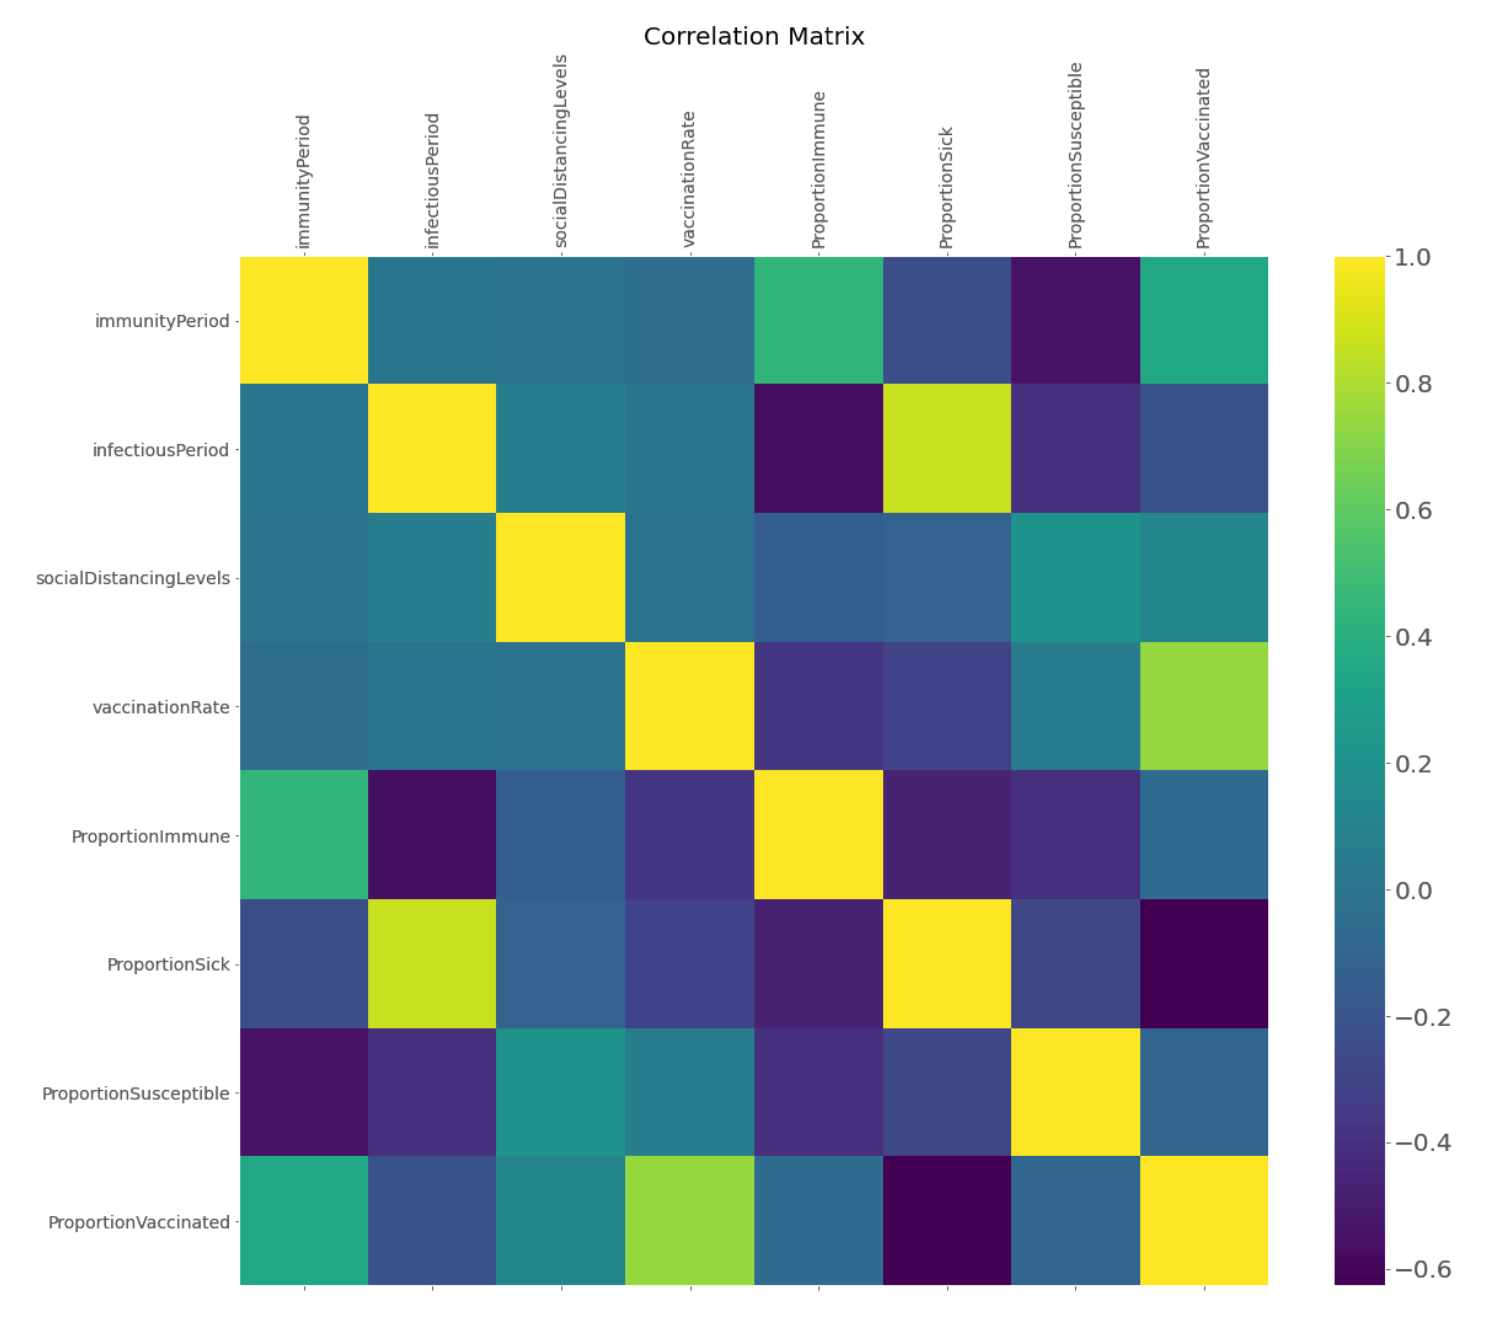
\includegraphics[width=0.7\linewidth]{figures/correlations.png}
	\caption{CORRELATION MATRIX OF THE MODEL PARAMETERS\label{fig:correlations}}
\end{figure}



%The correlation matrix illustrated in Figure 15 displays the correlation between different model parameters. The colour bar on the right side of the matrix visualises the intensity of the correlations between the parameters. The brighter the yellow, the higher the positive correlation and the darker the purple, the higher the negative correlation. The ‘ProportionSick’ and the ‘infectiousPeriod’ appear to be highly correlated. According to the box plots shown in Figure 14, every unit increase in the ‘infectiousPeriod’ also increased the ‘ProportionSick’ values. The rest of the input parameters, including the ‘immunityPeriod’, ‘socialDistancingLevels’ and ‘vaccinationRate’ are negatively correlated with the ‘ProportionSick’ at different intensity levels.

%The dependent variable of the regression summary shown in Figure 16 is the ‘ProportionSick’. All four input parameters of the model indicate significant p-values of zero, and the R-squared value is 93.7\%. The highest and the only positive coefficient among the four input parameters is between the ‘ProportionSick’ and the ‘infectiousPeriod’ by 0.0115. It indicates an increase in ‘ProportionSick’ by 0.0115 for every unit increase in the value of the ‘infectiousPeriod’. On the other hand, the coefficient values of the ‘immunityPeriod’, ‘socialDistancingLevels’ and ‘vaccinationRate’ are all negative by -0.0033, -0.0023 and -0.0041, respectively.


%In this research, we used multiple linear regression to estimate the relationship between the model’s input parameters and the proportional number of sick agents. A supplementary correlation matrix is drawn to visualise how strong the model parameters are correlated with each other. Then, a random forest model is trained with the original data obtained by the LHS method during the first step of the analysis to forecast the proportional number of sick agents.

%Before training the random forest model, the hyper-parameters of an estimator, which define the number of trees of the model, are firstly tuned by using the grid search method. After successfully training the random forest model, the predicted dataset is obtained and compared with the actual dataset on a density plot. Lastly, three different calculations, including MAE, MAPE, and RMSE, are conducted to determine how closely the predicted dataset fits the original dataset.

In order to train the random forest model to predict the values of the ‘ProportionSick’, the original data is categorised into train, test, and validation data in the ratio of 7:1.5:1.5. Before fitting the model with the train data, various numbers of trees with their corresponding accuracy scores are calculated and presented on a validation curve plot as shown in Figure 17. Then, the hyperparameter for the model was optimised using the grid search method for a given set of estimator values, including 800, 900, 950, 1000 and 1050. As a result, 900 is the best value for optimising the random forest model.

The random forest with the 900 decision trees was developed by fitting the training data to predict the values of the ‘ProportionSick’ and included the use of all four input parameters of the model. A partial random forest, of which the max depth is 4, is shown as an example in figure 18.

The predicted values of the 'ProportionSick' via the random forest are compared with the actual values in a table. The comparison between the statistical distributions of those two types of values is then visualised on a density plot.

The performance metrics in table 8 compare the predicted values to the actual values for the testing dataset. The first value refers to the MAE, which tells us how big of an error we can expect from the forecast on average (Error Metrics: How to Evaluate Your Forecasting Models, no date). The value we have here is merely 0.001, which implies that the average errors between the predicted and actual values are marginal; hence, the predictions are considered highly accurate. Moving on to the MAPE, the value of 0.363 indicates that, on average, the forecast is off by 0.363\%. This means that the accuracy of the forecast is as high as 99.637\%. Lastly, the value of the RMSE is also 0.001, which indicates that the difference between the predicted and actual values is marginal.

\begin{figure}
	\centering
	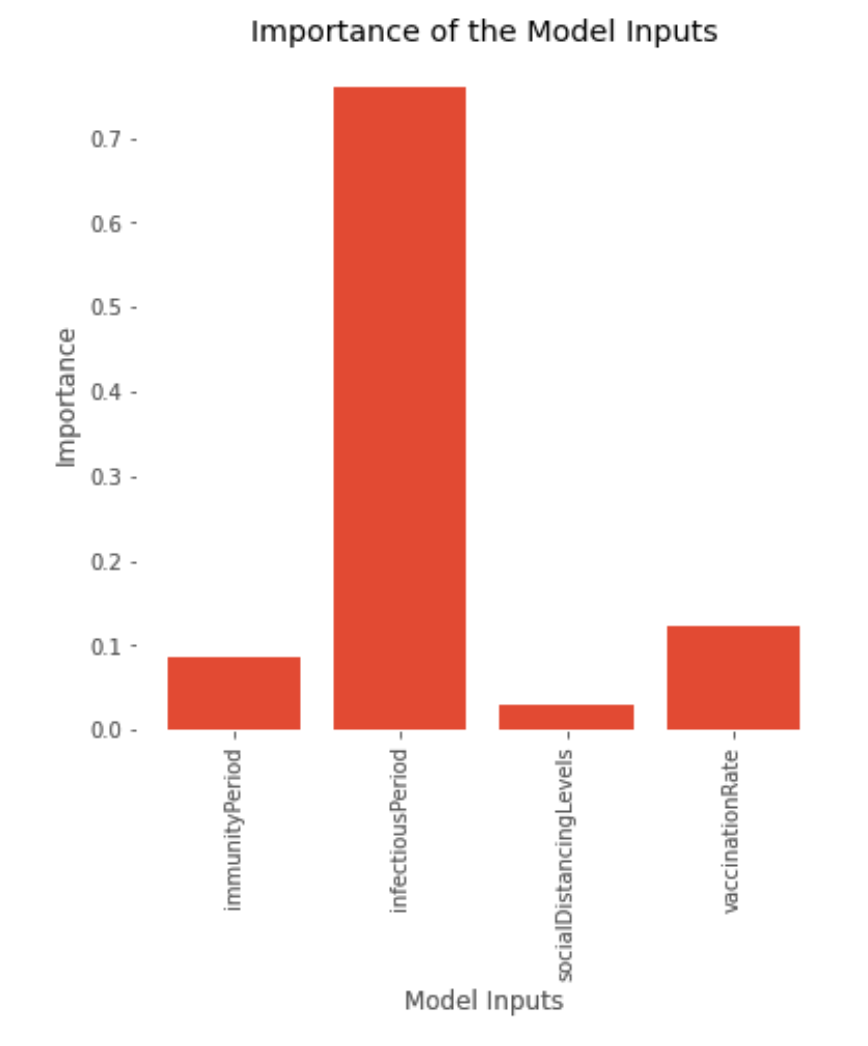
\includegraphics[width=0.5\linewidth]{figures/randomForest.png}
	\caption{FEATURE IMPORTANCE OF THE INPUT PARAMETERS GENERATED BY RANDOM FOREST MODEL\label{fig:randomForest}}
\end{figure}


The random forest model has quantified the importance of the model’s input parameters. The ‘infectiousPeriod’ is by far the most significant input parameter of the model, with a value of approximately 0.75. Followed by the ‘vaccinationRate’ with a value of slightly over 0.1. The ‘immunityPeriod’ and the ‘socialDistancingLevels’ had an importance rate below 0.1, which were not as significant as the previous two.


%4.4 Saltelli Sensitivity Analysis Results
\subsection{Global sensitivity analysis}


%3.6 Saltelli Sensitivity Analysis

%Saltelli is a statistical method for global sensitivity analysis which estimates sensitivity indices based on relative variances (Stastistical Sensitivity Analysis, 2022). The method decomposes the variances of the model’s output parameters into fractions that can be attributed to sets of input parameters. For instance, given a model that consists of two input and one output parameters, one might find that 50 percent of the output parameter variance is due to the variance in the first input, 30 percent to the variance in the second, and 20 percent due to the interactions between the two. These percentage values are indicative of the measures of sensitivity. Interpreting the results obtained from this analysis provides a better understanding of the relationship between the input and output parameters a model.
%There are two types of Sobol indices: the first-order Sobol sensitivity index and the total-order Sobol sensitivity index. The first one measures the direct effect each input parameter has on the variance of the model:
%𝑉(𝐸 (𝑌|𝑋)) 𝑆𝑖=𝑋𝑖𝑋~𝑖 𝑖 𝑉(𝑌)
% Where 𝐸𝑋~𝑖(𝑌|𝑋𝑖) indicates the expected value of the output 𝑌 when parameter 𝑋𝑖 is fixed. 𝑉 (𝐸 (𝑌|𝑋 )) measures the first-order index of 𝑋 on the model output in terms of variance 𝑋𝑖 𝑋~𝑖 𝑖 𝑖
%and is divided by the total variance, 𝑉(𝑌) for normalisation. Therefore, the result of the first-
%order Sobol sensitivity index shows the expected reduction in the variance of the model when the parameter 𝑋𝑖 is fixed. One thing to note is that the sum of the first-order Sobol sensitivity index cannot be bigger than 1.

%The total-order index, 𝑆𝑇𝑖, includes the first-order index and sensitivity due to all interactions between the given parameter, 𝑋𝑖, and other parameters of the model. 𝑉 (𝐸 (𝑌|𝑋 )) 𝑋~𝑖 𝑋𝑖 ~𝑖 𝑉(𝑌) Where, 𝑉 (𝐸 (𝑌|𝑋 )) refers to the first-order index of 𝑋 hence, 𝑉(𝑌) minus 𝑋~𝑖 𝑋𝑖 ~𝑖 ~𝑖 𝑉 (𝐸 (𝑌|𝑋 )) should give the value for the total-order index of 𝑋 . 𝑋~𝑖 𝑋𝑖 ~𝑖 𝑖 The Saltelli sensitivity analysis is available as the analytical tool on OpenMOLE. The programming script requires assigning the model’s input and output parameters with the number of samples defining the total model run. In this research, the number of samples is set to 60,000 for validation of the result.


In order to generate an accurate result for the sensitivity analysis, a total of 60,000 samples were run, as shown in figure 21.
25 days 7 hours = 25.29 days

\begin{table}
\caption{Saltelli total order indices}
\begin{tabular}{|c|c|c|c|c|}
Outputs & infectiousPeriod & immunityPeriod & vaccinationRate & socialDistancingLevels\\
ProportionImmune & 0.72 & 0.333 & 0.665 & 0.7\\
ProportionSick & 0.692 & 0.09 & 0.365 & 0.143\\
ProportionVaccinated & 0.516 & 0.319 & 0.587 & 0.337\\
ProportionSusceptible & 0.341 & 0.066 & 0.92 & 0.277\\
\end{tabular}
\end{table}

The total-order indices shown above indicate that the ‘infectiousPeriod’ has the most significant impact on the values of the ‘ProportionSick’ followed by the ‘vaccinationRate’, ‘socialDistancingLevels’ and ‘immunityPeriod’ respectively.




%4.5 NSGAII Results
\subsection{Multi-objective model optimisation}

In attempting to control the spread of epidemics, many problems involve multiple objectives which cannot simply be described as the more, the better or the lesser, the better; instead, each objective has an ideal target value, and the main goal is to reach the targeted value as close as possible. We have defined the model's four main input parameters for our research: the vaccination rate, infectious, immunity periods and social distancing. Based on one of the research questions, the goal is to find the optimal set of input parameters that can potentially suppress the spread of infectious diseases during the first year of the outbreak. To optimise the values of the input parameters, we define two objectives that are expected to be minimised. Firstly, we expect the proportional number of sick agents to be optimised, which is directly linked to the main interest of our research question. Secondly, we expect the proportional number of vaccinated agents to be optimised. Vaccination is a primary preventive measure that plays a vital role in successfully controlling the spread of diseases and even has the potential to achieve herd immunity, while other measures such as social distancing can only slow down the process of disease spreading instead of stopping them \cite{bicher2022model}. However, vaccines are not always available for multiple reasons, and one of the possible reasons might be due to the high manufacturing and transportation costs \cite{plotkin2017complexity}. This is where people like decision- makers often face a dilemma because attempting to control epidemics usually costs money and the best option which they might have at this point is to find a good balance between the usage of vaccines, which does not go over the budget, and the proportional number of sick agents.

The way to find the results that provide a good approximation of the Pareto frontier with acceptable trade-offs between the identified objectives is by using the NSGAII. The NSGAII is a commonly used type of multi-objective optimisation algorithm that consists of several unique characteristics. These characteristics include a fast non-dominated sorting, crowding distance assignment and sorting procedure \cite{deb2002fast}.

The Pareto Front consisting of non-dominated solutions relative to the ‘ProportionSick’ and ‘ProportionVaccinated’ is drawn after running a total of 10,000 samples.
3 days 19 hours = 3.79 days




\begin{figure}
	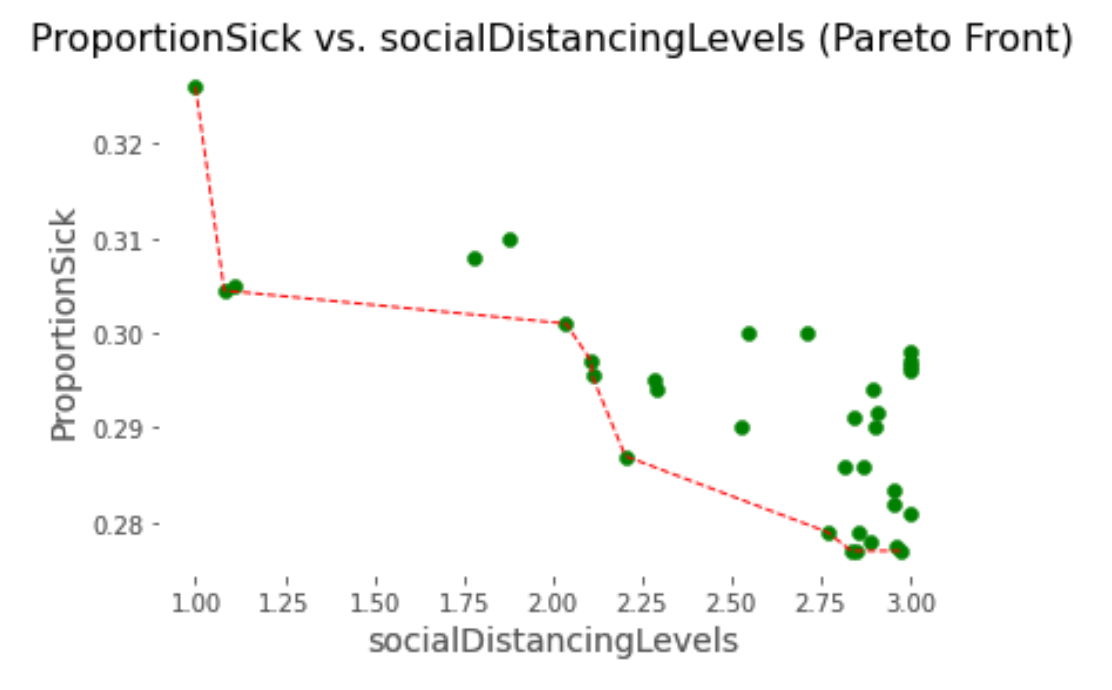
\includegraphics[width=\linewidth]{figures/pareto2.png}
	\caption{THE PARETO FRONT OF THE PROPORTIONSICK VS. VACCINATIONRATE\label{fig:pareto}}	
\end{figure}

The Pareto Front shown in Fig.~\ref{fig:pareto} illustrates the optimal solution set of the ‘ProportionSick’ and the ‘vaccinationRate’ as two objectives. The value of the ‘ProportionSick’ appears to decrease rapidly as the value of the ‘vaccinationRate’ increases. The slope of the line is generally steep throughout the graph. Plus, the difference between the values of the ‘ProportionSick’ with and without the vaccination is clear.


\begin{figure}
	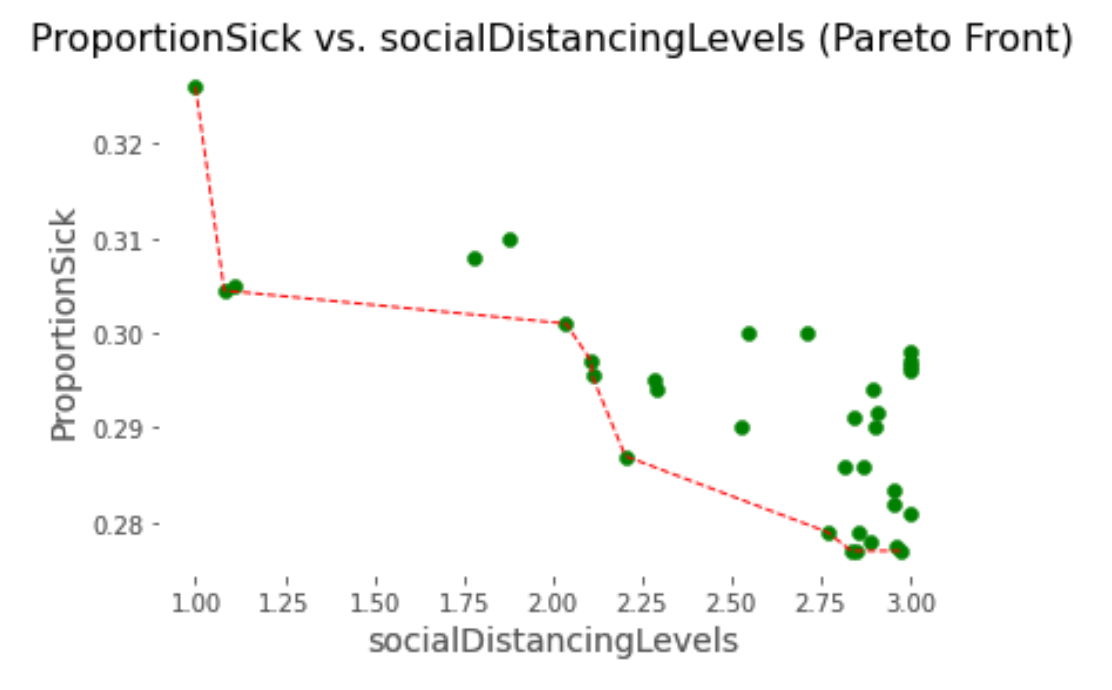
\includegraphics[width=\linewidth]{figures/pareto2.png}
	\caption{THE PARETO FRONT OF THE PROPORTIONSICK VS. SOCIALDISTANCINGLEVELS\label{fig:pareto2}}	
\end{figure}



The Pareto Front, visualised in figure 26, is formed with the optimal values of the ‘ProportionSick’ and the ‘socialDistancingLevels’ as two objectives. It indicates a clear sign of a decrease in the value of the ‘Proportionsick’ as the value of the ‘socialDistancingLevels’ increases.


\section{Discussion}

Overall, the spread of infection mainly depends on the longevity of the infectious period, according to the result obtained by the OLS regression analysis summary and the feature importance test in Figure 16 and 20, respectively. The longevity of the infectious period plays a vital role in disease transmission because a more extended infectious period allows an infected agent to interact with a more significant number of susceptible agents for an extended time. For example, an infected agent who is infectious for a single day is unlikely to infect a more significant number of susceptible agents than an infected agent who is infectious for a week. A more extended infectious period is, therefore, a dangerous factor that may rapidly increase the chances of infections, often creating a mass infection wave.
The vaccination rate is also a critical input parameter of the model that plays a vital role in controlling the spread of diseases because the vaccine is a significant source of protective measures that can effectively stop viruses from transmitting one agent to another \cite{storlie2021quantifying}. As mentioned in the literature review section, mass immunisation is the idealistic approach to herd immunity. This can be done by increasing the vaccination rate, thereby rapidly lowering the overall virus spread in the population.
According to the feature importance result shown in Figure 20, the importance of the immunity period and social distancing levels are marginal compared to the infectious period and the vaccination rate. However, synergies between them can further reduce the proportional number of sick agents. This idea can be supported by the results shown in Table 6 and 7, where the lowest proportional number of sick agents is obtained by the highest values of the immunity period, social distancing levels and vaccination rate. In contrast, the lowest values of those parameters resulted in the highest proportional number of sick agents. Furthermore, the total Sobol sensitivity indices for both the immunity period and the social distancing levels indicate significant values.
As mentioned, vaccines are essential, and probably the best preventive measure humans have found so far. However, once an agent gets infected, the infection process cannot be stopped with vaccines because they are not made for a cure. Instead, this is where other preventive measures such as social distancing, quarantine or even lockdown play essential roles in
55
mediating the spread of infectious diseases mainly by decreasing the contact rates between the agents while the vaccination process is taking place. The significance of the interaction between the immunity period and the social distancing level would not have been identified if the analysis was solely dependent on the feature importance result shown in Figure 20. Hence, the best approach to assessing the model’s input parameters is to apply various analytical methods to the data obtained. Also, to improve the overall synergistic effects of the preventive measures altogether, one way is by introducing additional preventive measures such as quarantine and lockdown to control infectious diseases better. By introducing more parameters into our model, there is a high chance of reducing the significance of the infectious period in terms of the total Sobol index. In other words, introducing more preventive measures can make the infectious period less significant in spreading diseases.
The cost of vaccines can be expensive, depending on one's economic state. As a decision maker, knowing the optimal solution to control the spread of diseases would be helpful in decision- making processes. The ideal goal would be to reach the highest value of the vaccination rate since it is the most effective preventive measure known. However, this would cost money and especially with a limited budget, one must remember that the most suitable optimal solution may not always be the highest vaccination rate. Based on the Pareto Front, we can estimate the cost spent on vaccines by referring to the proportional number of vaccinated agents and its corresponding impact can be indicated by the proportional number of sick agents on a trade-off curve.
The social distancing level is an essential input parameter that acts as a preventive measure against infectious diseases in our model. Social distancing must be implemented with care because if the intensity is too high, it prohibits necessary human interactions, which reduces the productivity rate, negatively impacting the economy in general (Emma, 2020). Due to this, finding a good balance between the social distancing level and the proportional number of sick agents would be essential in ensuring a healthy economy while keeping the number of infected cases low.


5.1 Limitations and Future Enhancements
Although this work has produced some meaningful results, it still poses some limitations and suggestions for future research. Firstly, the population size of the simulation had to be limited to a small number, mainly due to the expensive computational cost and time. For instance, running the current model, which takes about 35 to 40 seconds per run for 10,000 times, often costs several days to execute. In order to fasten the process, these executions have been separated into multiple clusters on OpenMOLE but still took several hours to run. The simulation duration with the number of initial agents has been fixed to limit the overall processing time. For instance, one tick which was initially equivalent to a minute in the simulation has been changed so that one tick is now equal to an hour. As a result, it costs only 24 ticks per day, while the former version used to cost 1440 ticks for a day to pass. Due to this, the duration of a day has been shortened, reducing the number of interactions between the agents. As a result, it might have affected the outcome of a simulation.
The current number of input parameters is limited to only four parameters. However, there can be more numbers of input parameters introduced in our model to generate more dynamic results which can better reflect real-life situations. Furthermore, the current model can be constructed with extra compartments that can describe various states of an agent in the infection process. If compartments such as death or exposure are added to the model, the states of an agent can further be categorised into a more significant number of states and make the overall dynamics of disease transmission rather sophisticated for an advanced result \cite{reyne2022principles}. The model is also flexible in that it can add many more characteristics of agents, such as age, occupation, vaccination record and gender, which can be considered in the process of interaction and infection. This will generate much more interesting results than the current model because considering more factors during the infection process may provide more sophisticated results that help humans better understand the overall dynamics of epidemics.



\section{Conclusion}

This study proposed various analytical approaches to assess the results obtained by the ABM, which has been built under the SIRV compartmental model to study the spread of diseases. Through the model, this study analysed the impacts of the pre-defined input parameters, which included the infectious period, immunity period, daily vaccination rate and social distancing level on the spread of infectious diseases. For analysis purposes, this research involved collecting and handling several model’s output parameters, including the proportional numbers of susceptible, infected, recovered, and vaccinated agents.
This research was divided into mainly five parts for the analysis of the results. Firstly, the input parameters’ values were randomly sampled via the LHS method to explore the model’s output space. Secondly, this research used a direct sampling method on the evenly spaced input parameter values to identify the combinations of the input parameter values that result in the lowest and highest proportional numbers of sick agents. Thirdly, the relationships between the model’s input parameters and the proportional number of sick agents were identified using the linear regression summary, and a prediction was made by training a random forest with the original data obtained. Fourthly, to analyse the sensitivity of the model’s input parameters, this research conducted the Saltelli global sensitivity analysis to decompose the variances of the model outputs into fractions that attribute to each of the model inputs. Lastly, using the NSGAII method, a Pareto Front consisting of optimal parameter values relative to the proportional number of sick agents was calculated.
It is proved in the research that the infectious period of an agent played the most crucial role in the spread of diseases, followed by the vaccination rate, immunity period and social distancing level, respectively. Furthermore, it is found that the lowest proportional number of sick agents is obtained by the lowest value of the infectious period with the highest values of the rest of the input parameters. According to the sensitivity analysis result, it is indicated that the infectious period dramatically impacts the total variance of the model outputs. However, the rest of the input parameters are also found to significantly affect the total variance of the model outputs, considering not just the impact done individually but also the impacts caused by interactions between them.

By referring to the Pareto Front, one may calculate the specific cost spent on vaccines and estimate the relative outcome based on the proportional number of sick agents. The social distancing levels would also cost economically depending on the level of its intensity; hence, the Pareto Front can be a good indicator tool for decision-makers to get a quick glimpse at how much each level of social distancing costs economically and its relative impact on the spread of diseases. Despite the research findings, there are some limitations and future enhancements regarding the research work. For the limitation, the number of ticks accountable for a single day had to be reduced so that each simulation consumes lesser computational power for the analysis to be carried out. As a result, this might have limited the chances of interactions between the agents. In terms of future enhancements, additional input parameters should be introduced to the model. This way, we can expect more sophisticated results since more features can be considered during the interaction and infection process.


\bibliographystyle{spphys}
\bibliography{biblio}

\end{document}
